\documentclass[letterpaper, 12pt]{article}
\usepackage[american]{babel}
\usepackage[utf8]{inputenc}
\usepackage[citestyle=apa,style=apa,backend=biber]{biblatex}
\usepackage[margin=1in]{geometry}
\usepackage{graphicx}
\usepackage{caption}
\usepackage{float}
\usepackage{array}
\usepackage{verbatim}
\setlength\bibitemsep{2\itemsep}
\DeclareLanguageMapping{american}{american-apa}
\addbibresource{bibliography.bib}

% my version of latex does not support this character apparently..
\DeclareUnicodeCharacter{2212}{-}

\begin{document}
\begin{titlepage}
\centering
	\vspace*{5.75cm}
	{\huge\bfseries Mini S08\par}
	{\large ECE 643 Final Project\par}
	\vspace{2cm}
	Dan Wagner\\
	Kansas State University\\
	College of Engineering\\
	Department of Electrical and Computer Engineering\\
	\vspace{1cm}
	Dr. John Devore\\
	Professor\\
	Department of Electrical and Computer Engineering\\
	\vspace{1cm}
	December 8, 2017
\end{titlepage}

\section*{Introduction}
\thispagestyle{plain}
The Mini S08 project was designed to emulate a subset of instructions from the Freescale S08 microcontroller on an Altera DE2 FPGA development board.  The subset was thorough and allowed the Mini S08 to function exactly like the microcontroller except for a few instructions (such as the cmp instruction) in order to keep the project simplistic.
The Mini S08 was constrained to be coded in either the Verilog or AHDL languages.  The seven segment displays on the board were also required to be used for displaying the Instruction Register, Data Bus, and Address Bus values.


~\newline
A Floating Point Unit (FPU) was incorporated into the project to perform two operations: division and multiplication.  The Mini S08 was able to take two IEEE 754 Floating Point numbers and perform a division and/or multiplication on them.  The FPU was built upon the project's previous functionality, as the core framework was completed.


\begin{flushleft}
~\newline
\section*{IEEE 754 Standard}
The IEEE 754 Floating Point Standard [1] specifies the format of 32-bit floating point numbers.  Each number adheres to the following format:
~\newline
\begin{enumerate}
	\item The most significant bit is the sign bit which is true when the number is negative.
	\item The next eight bits are the biased exponent bits. The bias is 127.
	\item The remaining 23 bits are the normalized fractional bits of the number.
\end{enumerate}

When performing arithmetic, the end result may require rounding.  Two main methods were investigated: round to even and round to odd.  In round to even, the number is rounded as to make the least significant bit a zero (rounds to the nearest even number).  If round to odd is used, the least significant bit of the number is made to be a one (rounds to the nearest odd number).

\newpage
\section*{Data Flow}

The data flow consists of several components and can be seen in the following figure.
 \begin{figure}[H]
 	\centering
 	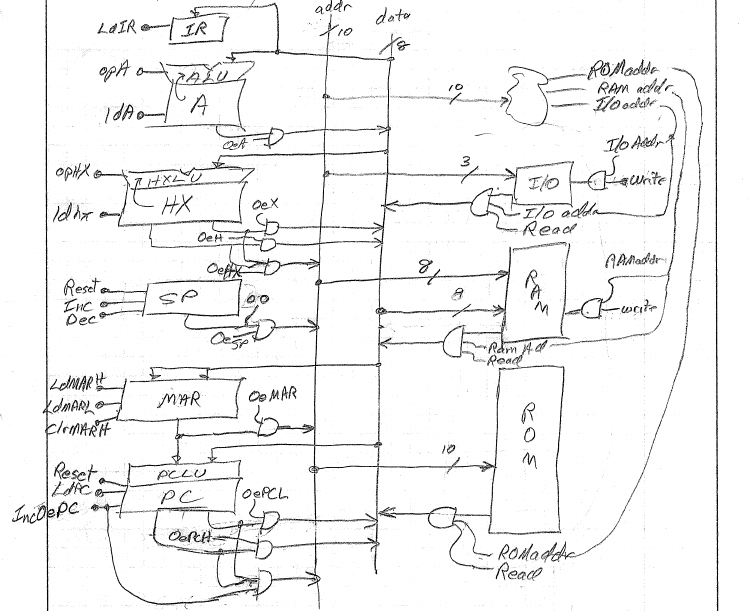
\includegraphics[width=\linewidth,height=10cm,keepaspectratio]{dataflow.png}
 	\caption[Mini S08 Data Flow]{Data Flow of the Mini S08 Project (excluding FPU).}
 	\label{fig:arch}
 \end{figure}

The Mini S08 contains two buses for information: an 8-bit data bus and a 10-bit address bus.  The address bus is ten bits to accommodate the ROM memory space size.  Information on the address bus pertains to memory locations where the program or registers need to access in order to retrieve the required information.  Data bus accesses are for transporting pieces of data found at these locations, or directly given (in the case of Immediate addressing).

~\newline
Each register obtains their values from the data bus in different forms.  The accumulator (A) is fed its value from the arithmetic and logic unit (ALU), which gets its value from the bus.  The H:X register pair obtains its value in a similar fashion, as does the Program Counter (PC).  Finally, the Memory Address Register (MAR) pulls its data directly from the bus.

~\newpage
Interaction with the address bus are more complicated.  The information placed on this bus depends upon the addressing mode and the specific instruction.  In Indexed addressing, the data the instruction needs is located in the memory location denoted by the HX register; thus, the HX register is put onto the address bus.  Immediate and Relative addressing access the memory location pointed at by the PC, while Direct accesses the location pointed at by the MAR. Stack addressing and the rts instruction retrieves data from the location pointed at by the Stack Pointer (SP).

~\newline
Input and output are coordinated between the buses and four modules: FPU, RAM, ROM, and SCI.  In Figure 1, the FPU is not shown, and the SCI module is renamed I/O.  Data flows to these modules from the address bus (accessing these modules requires addressing each).  These modules transfer information to the data bus to be used by the program.

~\newline
The control signals coordinating these transactions will be discussed in the next section.

~\newpage
\section*{Control Units}
The Mini S08's operation was modeled as a state machine with five states.  These states are shown in Figure 2.
 \begin{figure}[H]
 	\centering
	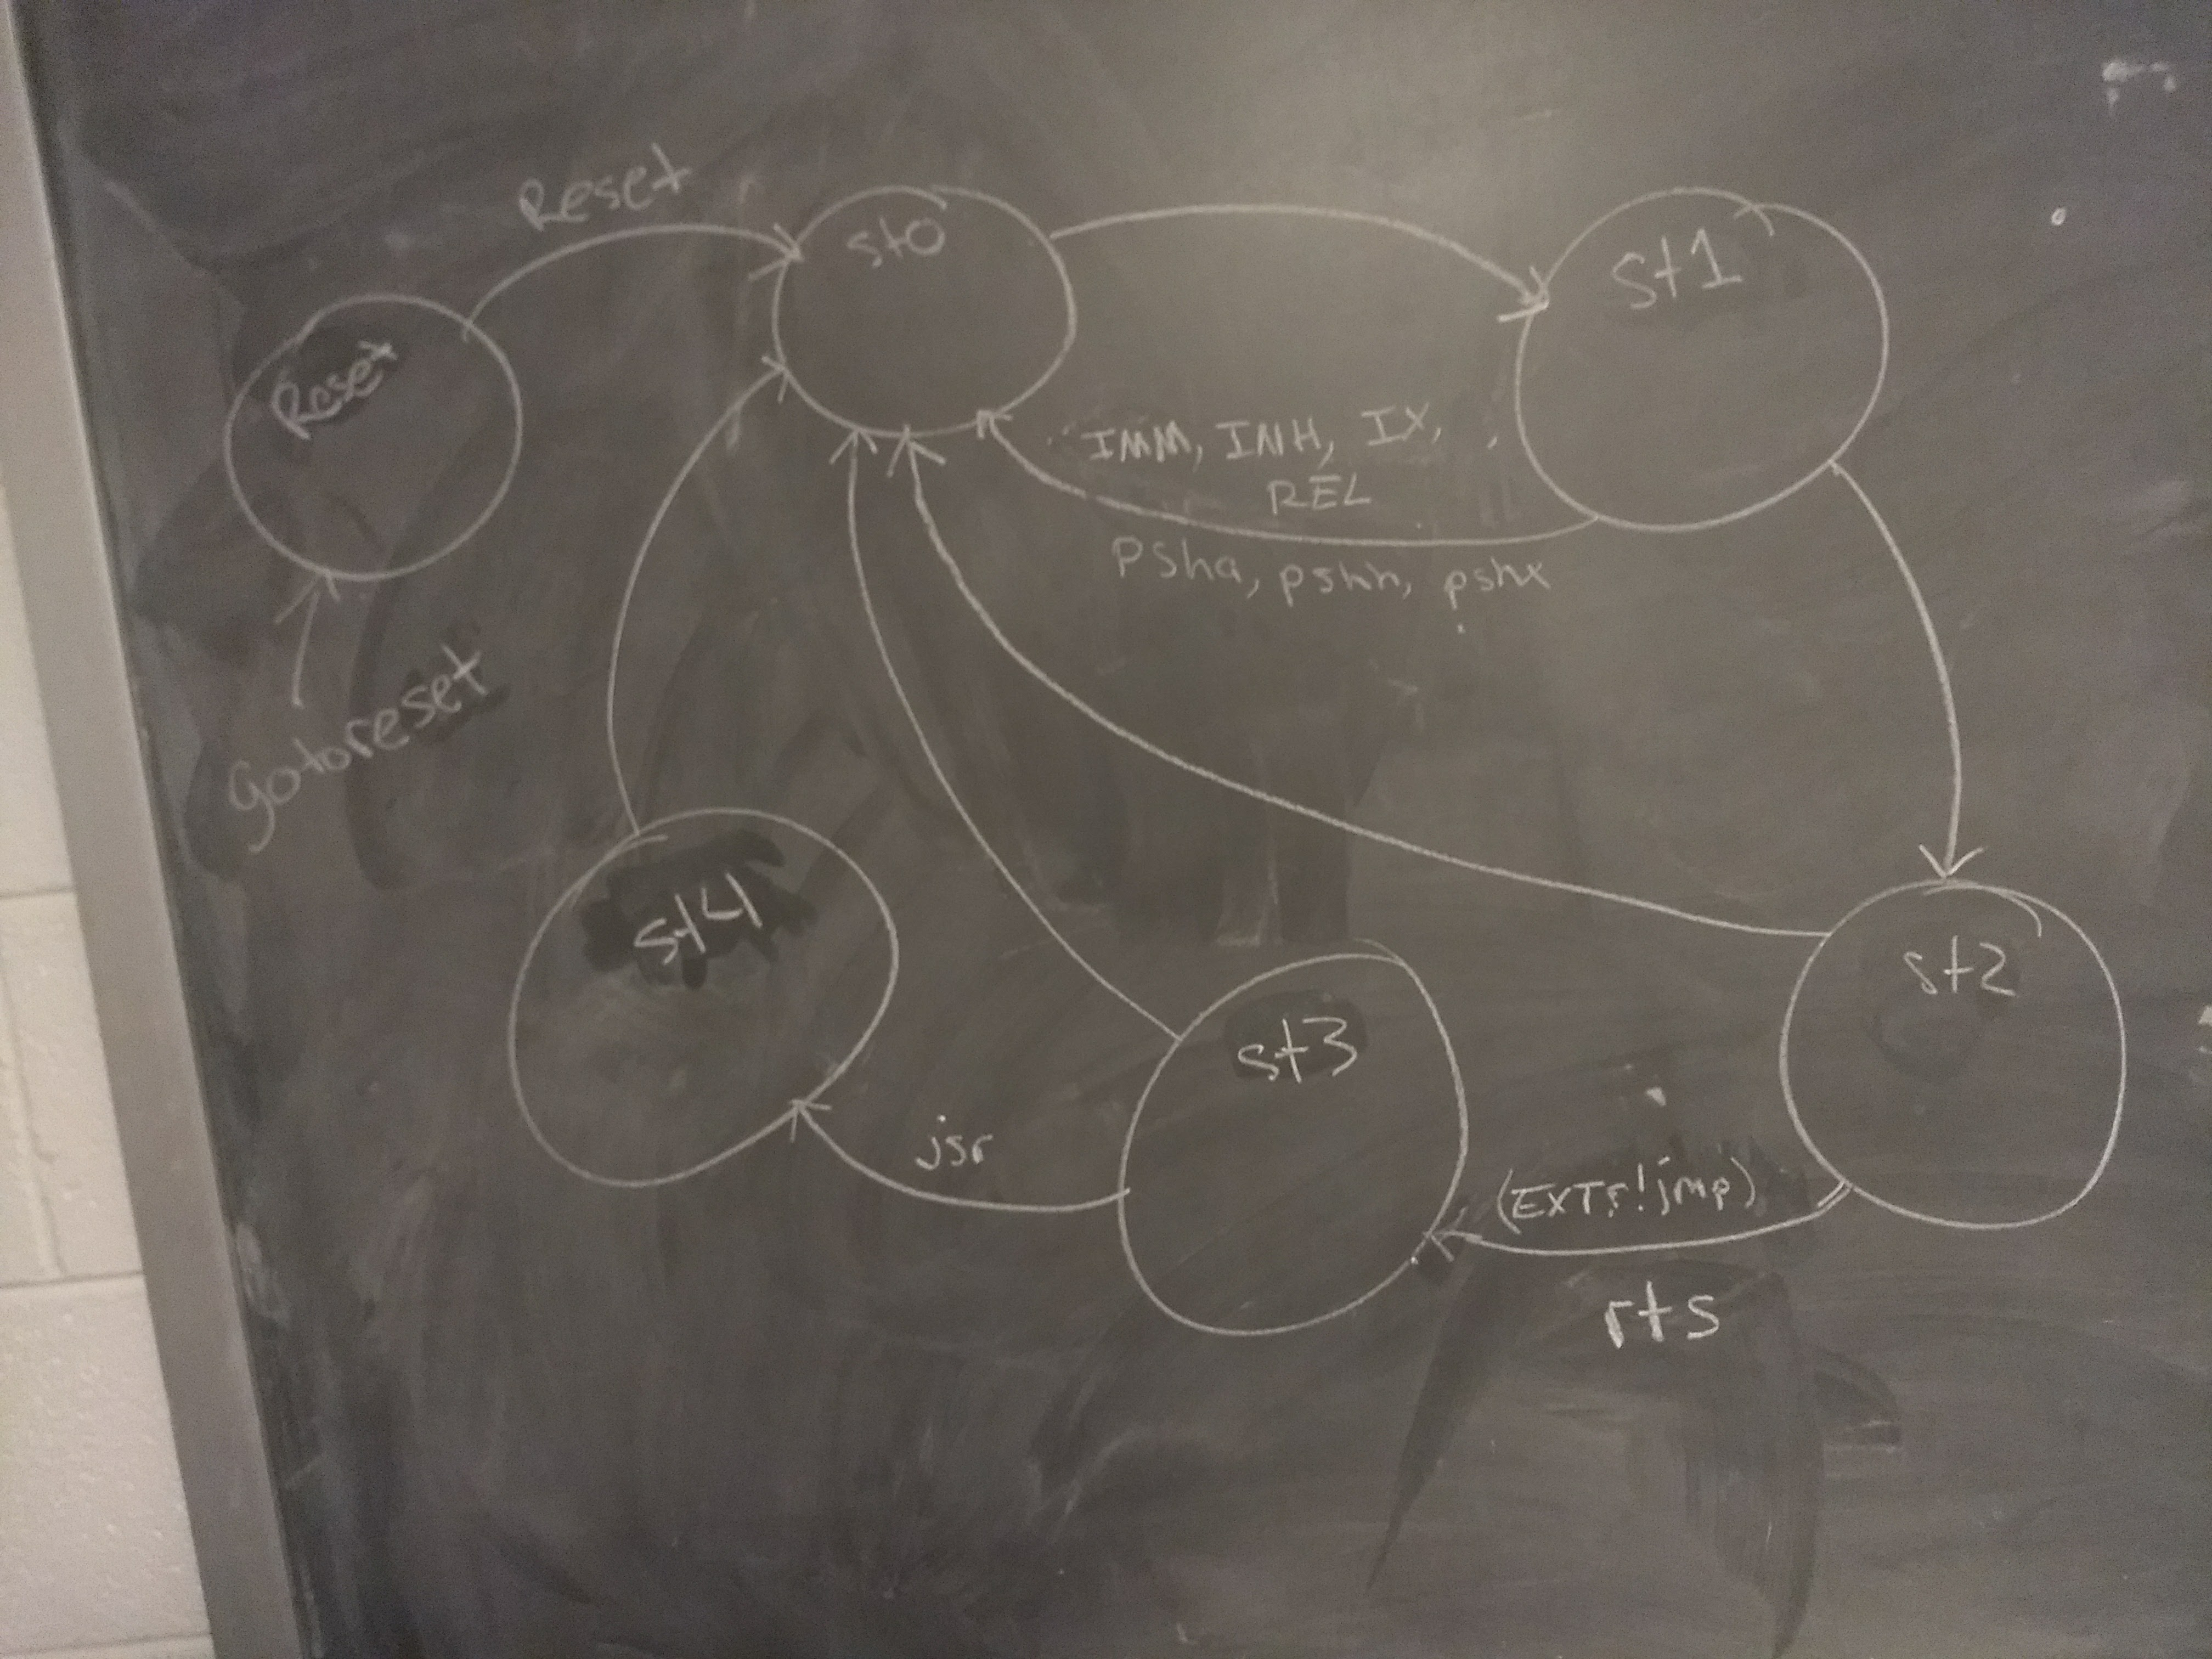
\includegraphics[width=\linewidth,height=10cm,keepaspectratio]{s08_states.jpg}
	\caption[Mini S08 State Machine Diagram]{State Machine for the Mini S08 Project.}
	\label{fig:arch}
\end{figure}

%Talk about the transitions and state diagram here.
Reset is the initial state that the MiniS08 is in when programmed.  When the reset push button is pressed, the program returns to this state and transitions to state zero. State zero is where the instruction is fetched into the IR.  After fetching, the next state is state one.

~\newline
State one decodes the fetched instruction and transitions to different states depending on the address mode.  If the instruction is an Immediate, Inherent, Indexed, Relative, or one of the push instructions, then the instruction is completed in one cycle and the system transitions to the state zero.  Otherwise, additional cycles are required for complete the execution and flow transitions to state two.

~\newline
State two continues executing instructions that failed to take one cycle to complete.  If the instruction is an Extended or jmp instruction, or an rts instruction, then another state is required to complete it (state three).  Otherwise, the instruction finishes and the system transitions back to state zero.

~\newline
State three, similar to state two, resumes instruction execution that failed to complete in the prior state(s).  Most instructions finish executing here, but jsr requires transitioning to the final state.

~\newline
State four is required for the jsr instruction, as it requires four cycles to complete.  After completion, the system transitions back to state zero.

~\newline ~\newline
The diagram in Figure 2 fulfilled the operating requirements for the S08 without the FPU.  When the FPU was added to the project, two additional state diagrams were required: one for multiplication, and one for addition.  Shown below, the multiply state machine required three states depending on the operation's result.

 \begin{figure}[H]
 	\centering
	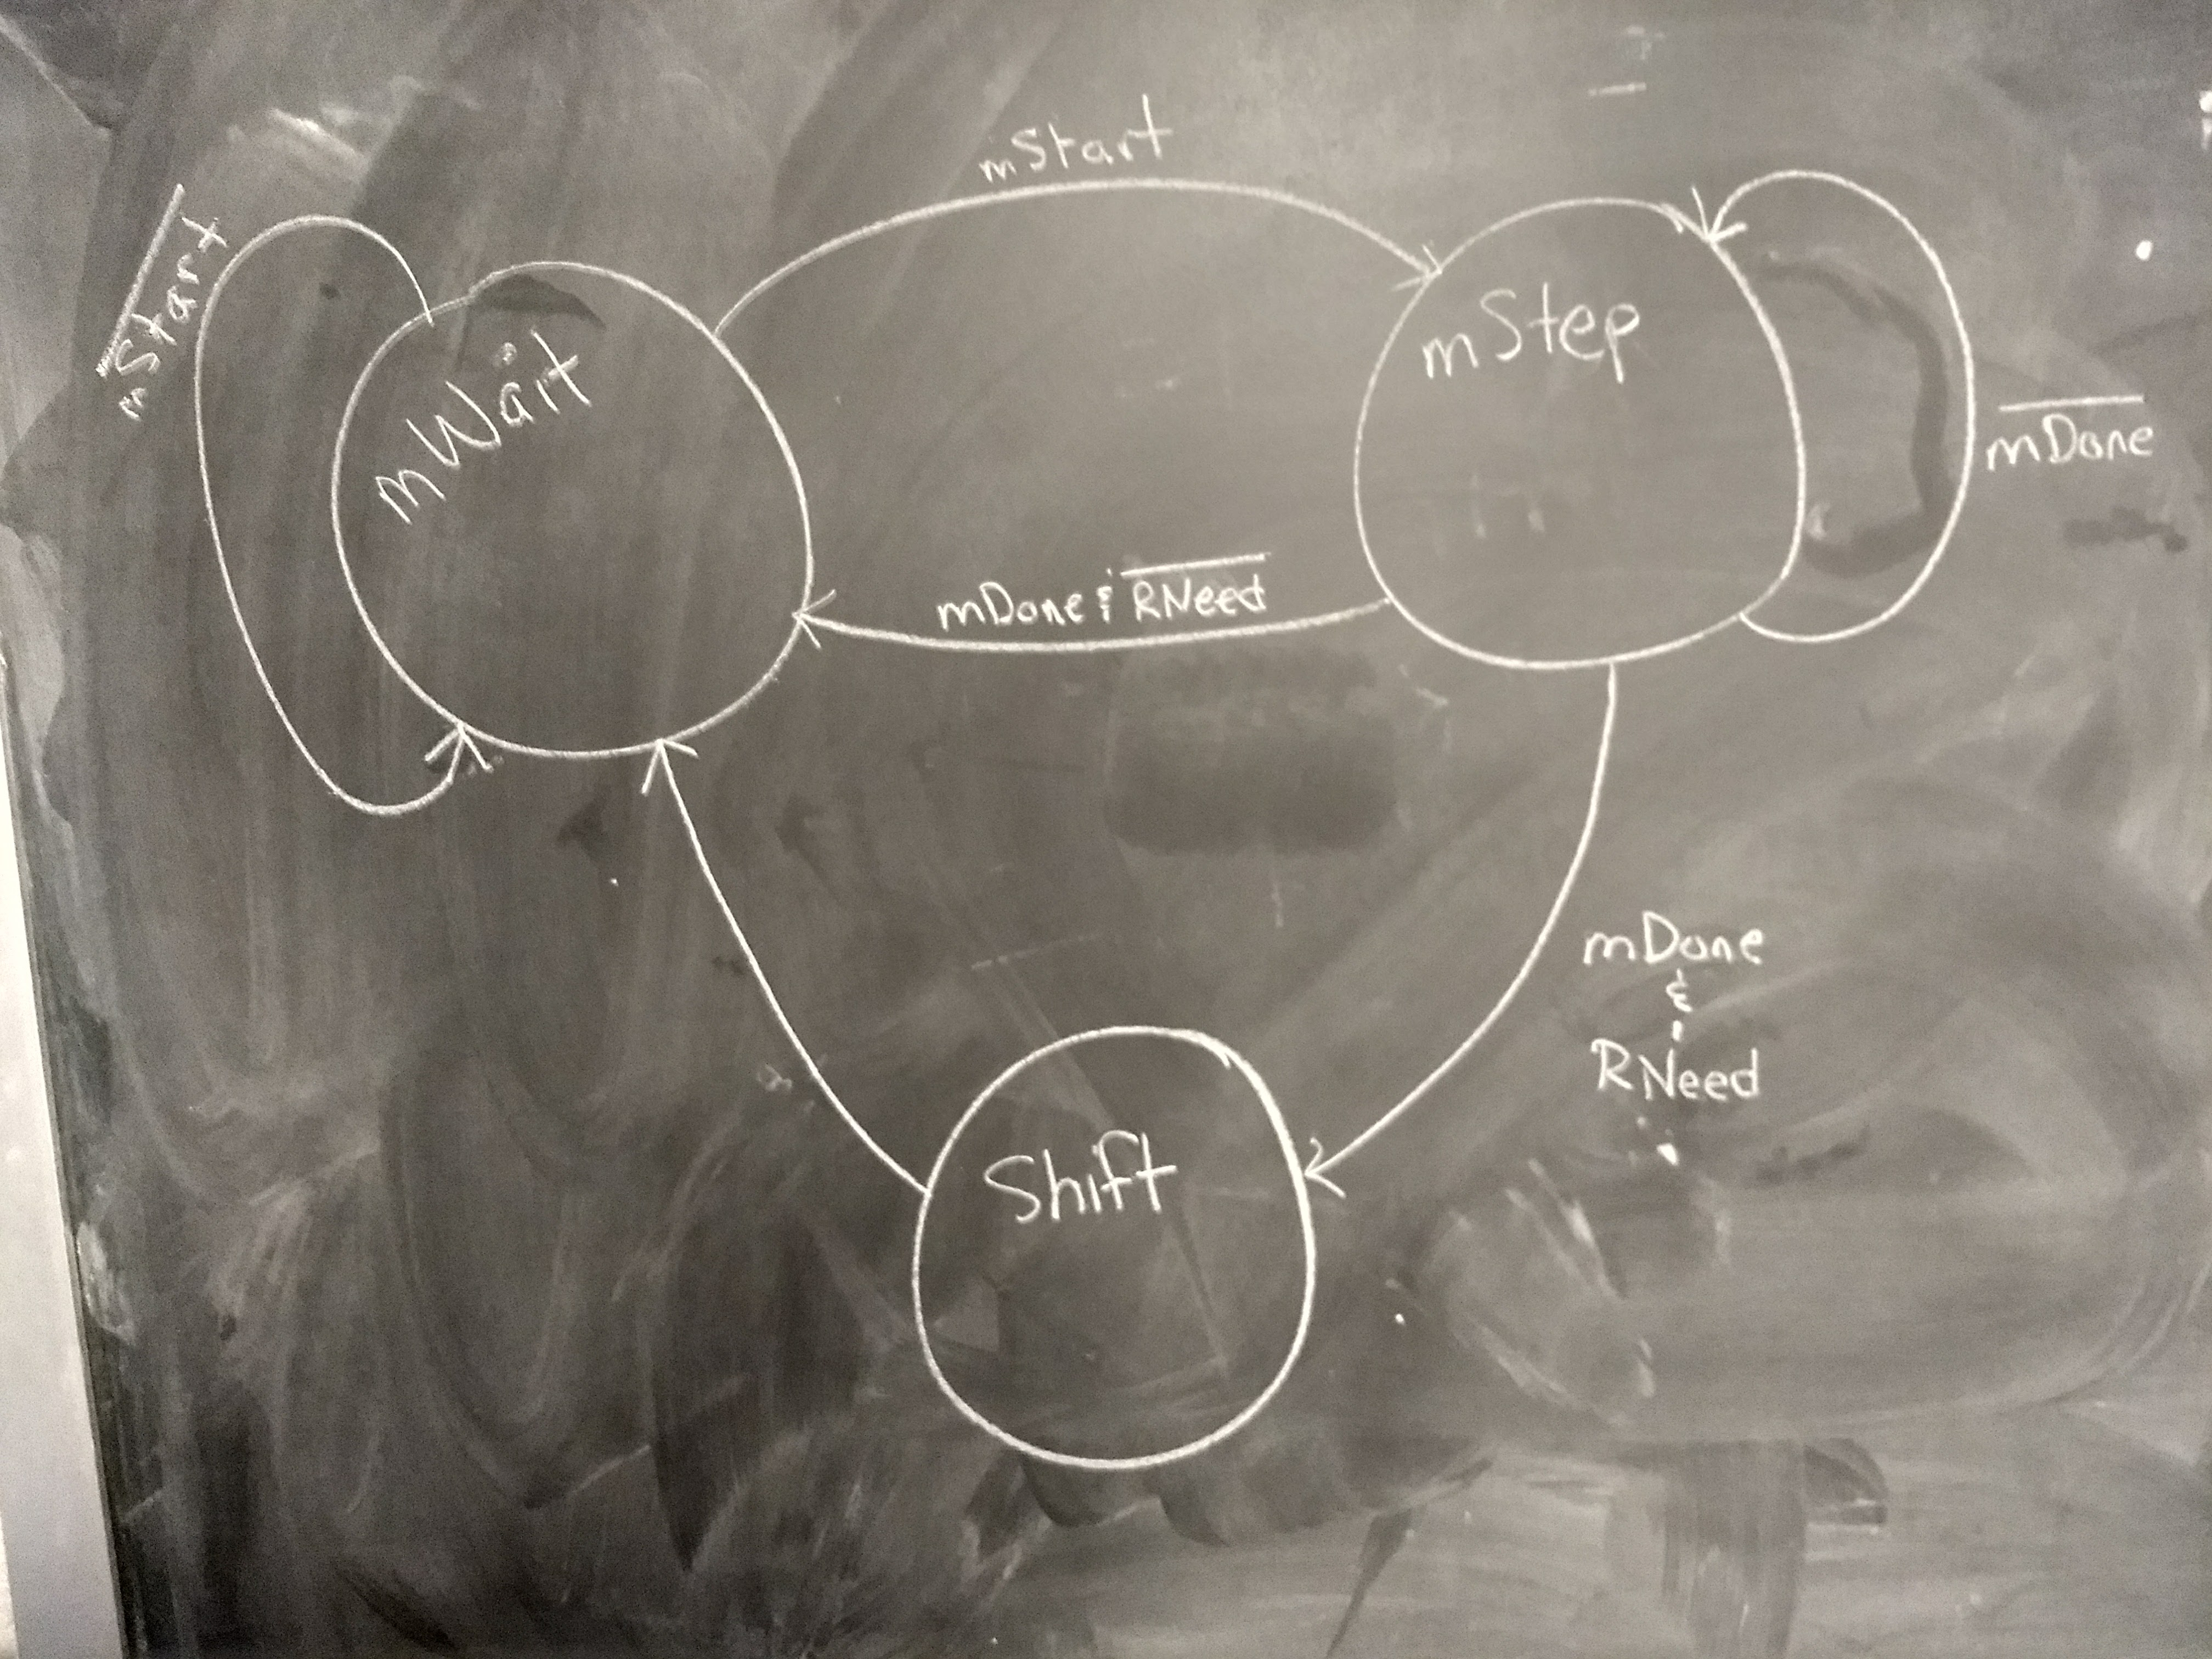
\includegraphics[width=\linewidth,height=10cm,keepaspectratio]{multiply_states.jpg}
	\caption[Mini S08 Multiply State Machine Diagram]{Multiply State Machine for the Mini S08 Project.}
	\label{fig:arch}
\end{figure}

The multiply state machine begins in the waiting state.  The FPU waits for all data to be input from the S08 before beginning the operation.  The FPU receives both numbers to multiply and the operation to perform from the S08 data bus.  Once all information is received, the start signal enables and the system transitions to the step state.

~\newline
Most of the work is done within the step state.  On each iteration, a portion of the multiplication is performed (mainly, shifting and adding).  The system remains in this state until the multiplication operation is complete.  If rounding is required, the system transitions to the shift state and shifts the product right by one bit.  Otherwise, it returns to the waiting state and the cycle begins anew.

\newpage
The division state machine is simpler than either the multiplication or S08 machines.  It consists of two states, as shown in Figure 4.

 \begin{figure}[H]
	\centering
	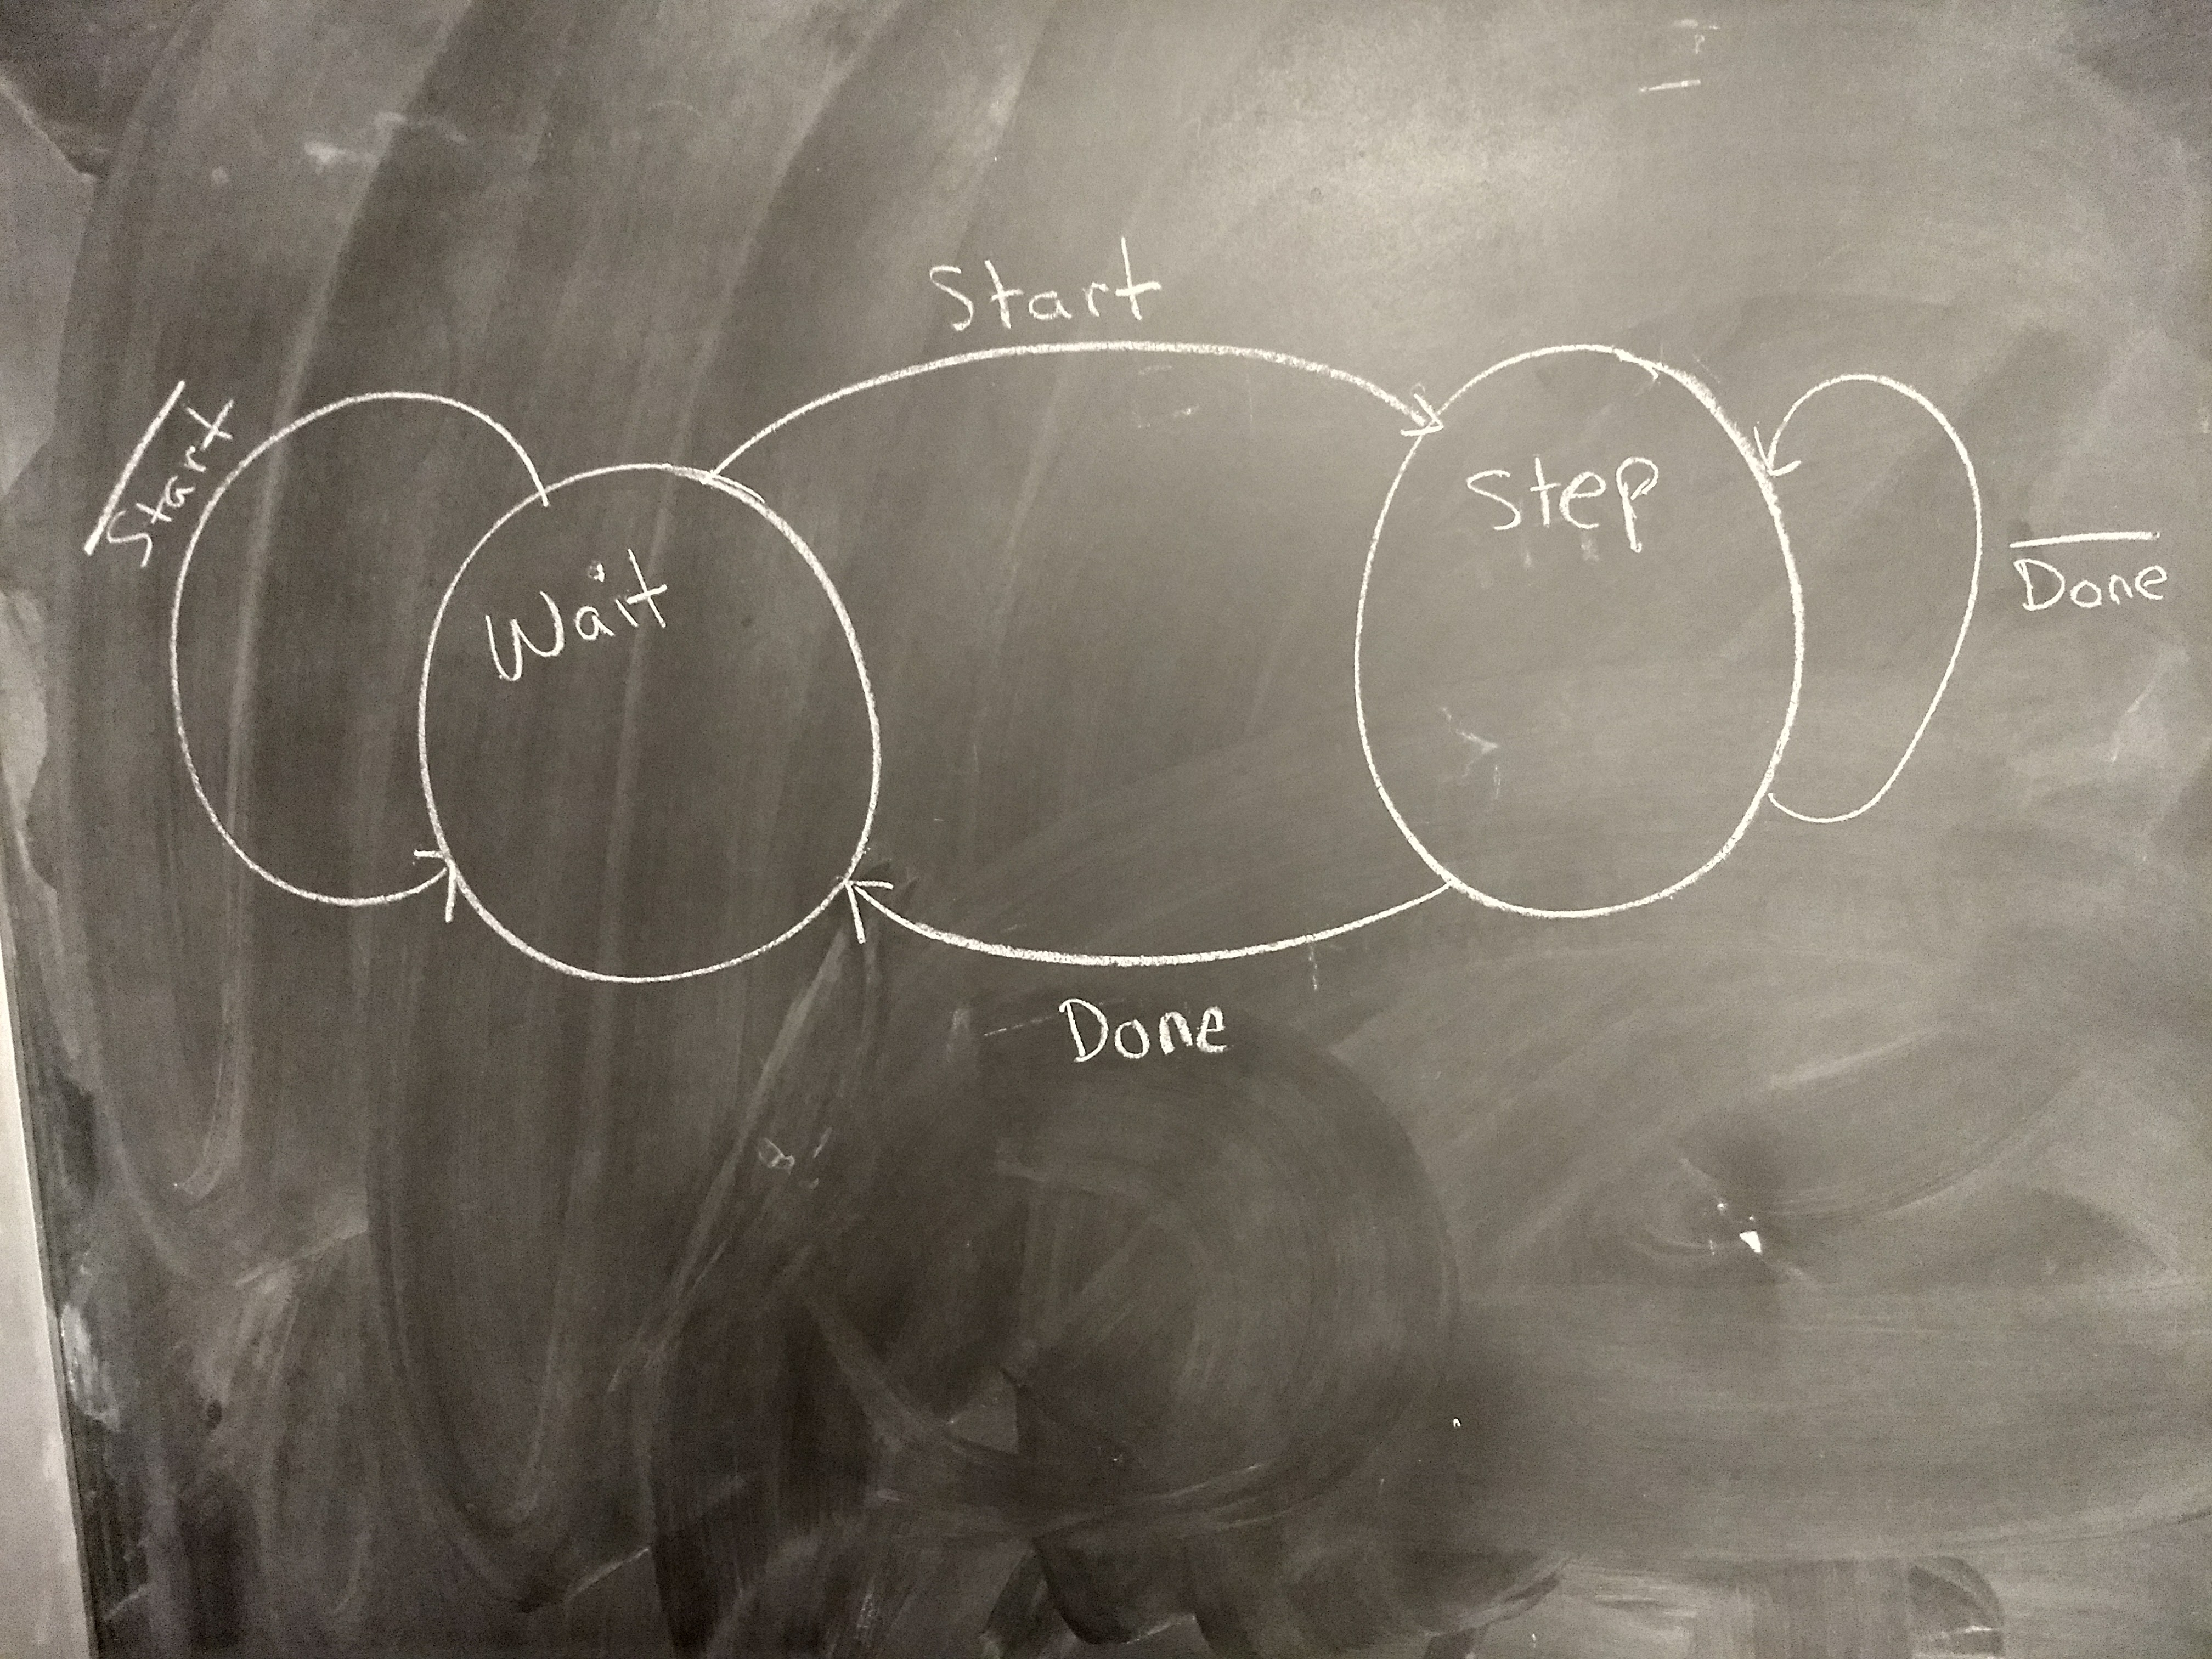
\includegraphics[width=\linewidth,height=10cm,keepaspectratio]{divide_states.jpg}
	\caption[Mini S08 Division State Machine Diagram]{Divide State Machine for the Mini S08 Project.}
	\label{fig:arch}
\end{figure}

The system remains in the waiting state like the multiply state. It waits for both floating point values and the operation to be entered.  Once these requirements are met, the system transitions into the step state.

~\newline
Very similarly to the multiplication operation, the step state is the main working state for division.  On each iteration, a portion of the operation is completed.  This state remains the active state until the division is completed.  At this point, any required rounding is performed and the system transitions back to the waiting state.

\newpage
\section*{Conclusion}
The project was an overall success, as seen in the Figures 5-8.
 \begin{figure}[H]
	\centering
	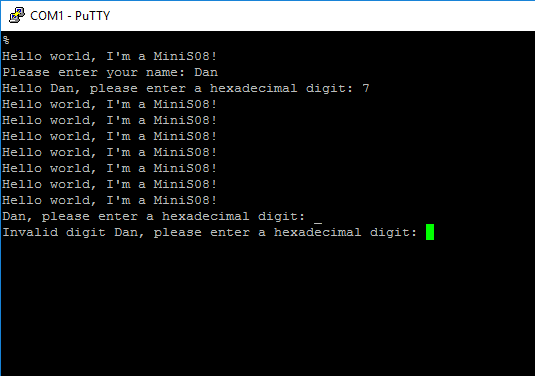
\includegraphics[width=\linewidth,height=10cm,keepaspectratio]{minis08_operation.PNG}
	\caption[MiniS08 Operation Proof]{Proof of Mini S08 Functionality.}
	\label{fig:arch}
\end{figure}

Initially, the project was daunting and required more work than thought.  Writing the register transfer notation (RTN) statements was simple from the data flow diagram provided.  Programming with Verilog and translating those statements proved another challenge, as the Altera Quartus II software enjoyed automatically optimizing code fragments away.  These optimizations resulted in bugs when testing and were usually resolved by fixing a variable declaration or logic error.

~\newline
The project is an excellent example of the overall design process of a computer.  First, we started with the data flow and configuring how to accomplish and coordinate the data lines.  From there, we developed the RTN.  Then, we translated the statements into Verilog and debugged the result.  Finally, we had our working computer.

~\newline
The only major change I would recommend is moving away from the Quartus II IDE.  It is not very useful with a majority of the bugs that we were facing (auto-optimization) and was not helpful when debugging.
 \begin{figure}[H]
	\centering
	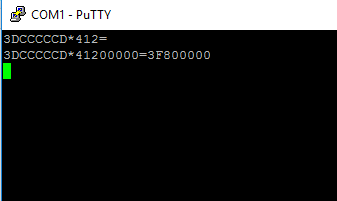
\includegraphics[width=\linewidth,height=10cm,keepaspectratio]{multiplication_fpu.PNG}
\caption[MiniS08 Multiplication Proof]{Proof of Mini S08 Multiplication.}
	\label{fig:arch}
\end{figure}
 \begin{figure}[H]
	\centering
	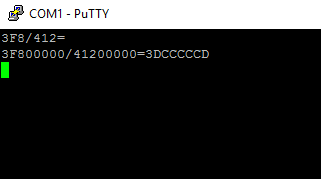
\includegraphics[width=\linewidth,height=10cm,keepaspectratio]{division_fpu.PNG}
\caption[MiniS08 Division Proof]{Proof of Mini S08 Division.}
	\label{fig:arch}
\end{figure}
\newpage
\section*{References}
1. IEEE Standard for Binary Floating-Point Arithmetic IEEE Std. 754-2008, 2008. 

\newpage
\section*{Source Code: S08}
\verbatiminput{minis08.v}
\newpage
\section*{Source Code: FPU}
\verbatiminput{fpu.v}
\end{flushleft}

\end{document}
